\section{La onda}\label{sec:la-onda}

Para la física, una onda consiste en la propagación de una perturbación de energía sin transporte de materia.

La magnitud física cuya perturbación se propaga se expresa como una función tanto de la posición como del tiempo
$\psi(\vec{r},t)$.

Matemáticamente se dice que dicha función es una onda si verifica la ecuación de ondas:
\begin{equation}\label{eq:ecuacion-onda}
\nabla^2\psi(\vec {r},t)=\frac {1}{v^2}\frac{\partial^2\psi}{\partial t^2}(\vec {r},t)
\end{equation}
donde $v$ es la velocidad de propagación de la perturbación.

\subsection{Elementos de una onda}\label{subsec:elementos-de-una-onda}

\begin{description}
    \item[Cresta.] El punto de máxima separación con respecto de su posición de reposo.
    \item[Valle.] El punto de máxima elongación de la onda, en sentido opuesto a la cresta.
    \item[Amplitud ($A$).] La distancia vertical desde una cresta hasta el punto de equilibrio.
    \item[Longitud de onda ($\lambda$).] La distancia entre dos crestas consecutivas.
    \item[Número de onda angular ($k$)]. La inversa de la longitud de onda en radianes.
    \item[Periodo ($T$).] El tiempo empleado en completar una longitud de onda.
    \item[Frecuencia ($\nu$).] El número de periodos por unidad de tiempo.
    \item[Frecuencia angular ($\omega$).] La frecuencia en radianes por segundo.
    \item[Fase ($\alpha$).] El mínimo valor que hace cíclica la posición.
    \item[Velocidad de fase ($v_f$).] La velocidad a la que se propaga el movimiento ondulatorio.
    \item[Velocidad de grupo ($v_g$).] La velocidad a la que se propaga las variaciones de la amplitud.
\end{description}

Aplicando las definiciones anteriores, tenemos: $k=\frac{2\pi}{\lambda}$, $\nu=\frac{1}{T}$,
$v_f=\frac{\lambda}{T}=\nu\lambda$ y $\omega=2\pi\nu$.

\begin{figure}[b]
    \centering
    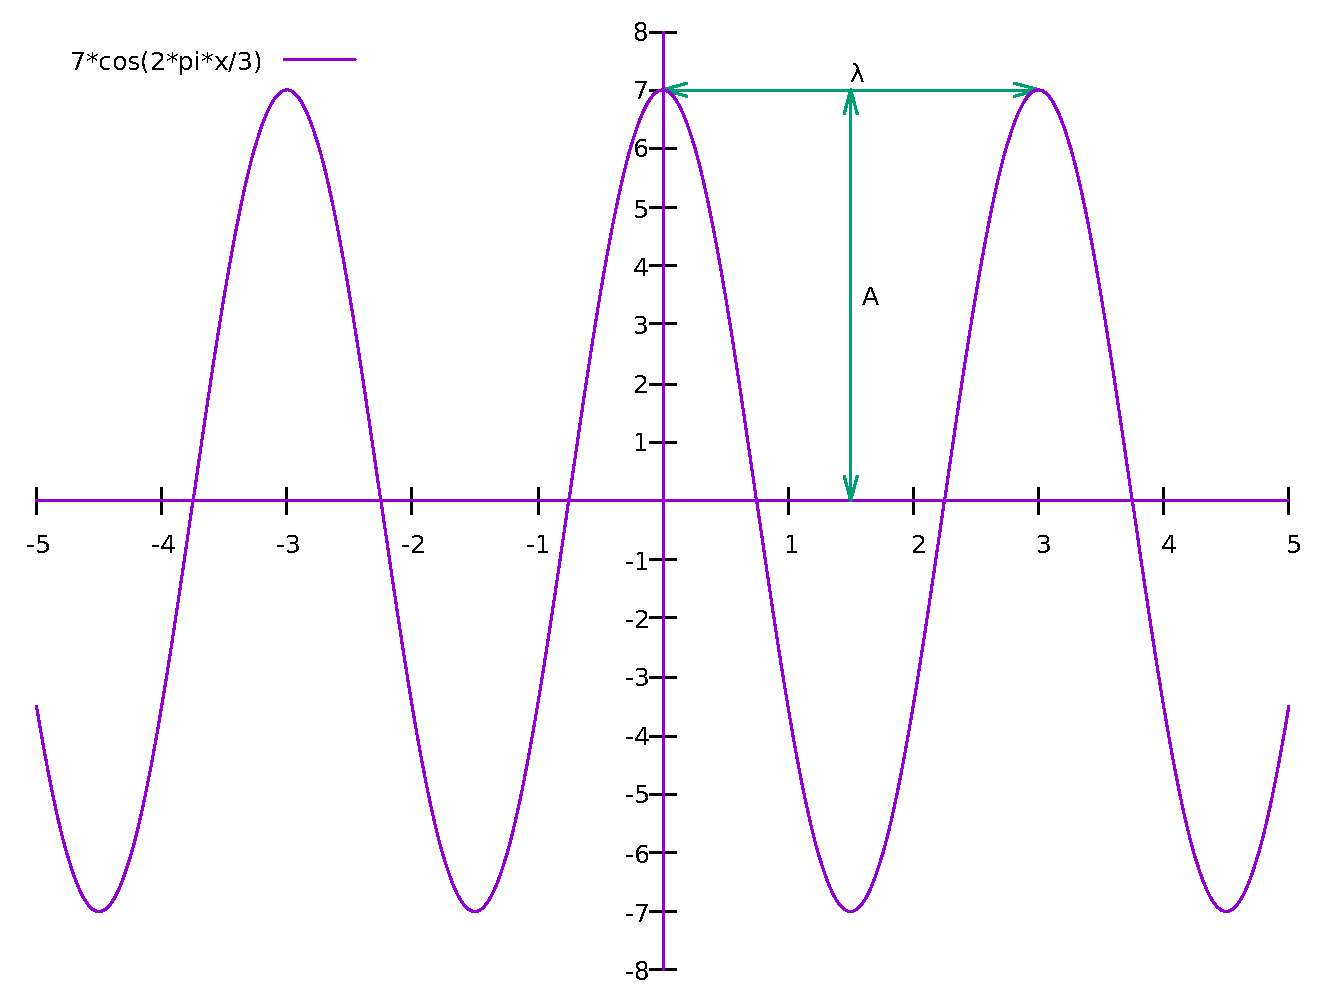
\includegraphics{coseno.pdf}
    \caption{Elementos de una onda}
    \label{fig:elementos-onda}
\end{figure}

\subsection{Soluciones a la ecuación de onda}\label{subsec:soluciones-a-la-ecuación-de-onda}
La solución más sencilla a la ecuación de ondas es considerar una onda plana que se desplaza longitudinálmente en la
dirección de la onda, donde si situamos el sistema de referencia en un punto de equilibrio tenemos la solución:
\begin{equation}
    \label{eq:solucion-ecuacion-ondas-simple}
    \psi(x,t)=A(x,t)\sin(\omega t-kx)
\end{equation}

\section{Dualidad onda-partícula de De Broglie}\label{sec:dualidad-onda-partícula-de-de-broglie}

Si los fotones son partículas y ondas a la vez, podemos usar el postulado de la mecánica relativista para partículas
con masa, donde la energía de una partícula es $E=m c^2$, y a la vez, usar el resultado de Planck sobre las energías
de una onda, donde $E=h\nu$. Así pues igualando ambas energías se tiene que $m c^2=h\nu$, pero como la velocidad de
una onda es igual al producto de la frecuencia y la longitud de onda, tendremos que:
\begin{equation}
    \label{eq:dualidad-onda-particula}
h\nu = m c^2 = m c c = p \nu\lambda\so h = p\lambda\so \lambda = \frac{h}{p}
\end{equation}